


\tikzset{every picture/.style={line width=0.75pt,scale=0.6}} %set default line width to 0.75pt        

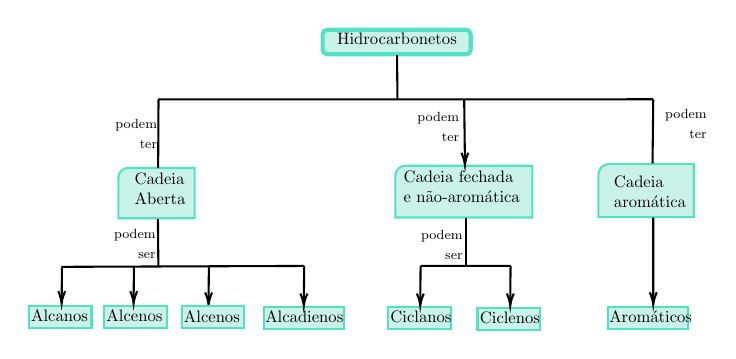
\begin{tikzpicture}[x=0.75pt,y=0.75pt,yscale=-.9,xscale=.85, every node/.style={scale=0.6}]
	%uncomment if require: \path (0,352); %set diagram left start at 0, and has height of 352
	
	%Rounded Rect [id:dp10752643749249613] 
	\draw  [color={rgb, 255:red, 80; green, 227; blue, 194 }  ,draw opacity=1 ][fill={rgb, 255:red, 203; green, 242; blue, 233 }  ,fill opacity=1 ][line width=1.5]  (297.63,34.71) .. controls (297.63,32.29) and (299.59,30.33) .. (302.01,30.33) -- (433.21,30.33) .. controls (435.62,30.33) and (437.58,32.29) .. (437.58,34.71) -- (437.58,47.84) .. controls (437.58,50.25) and (435.62,52.21) .. (433.21,52.21) -- (302.01,52.21) .. controls (299.59,52.21) and (297.63,50.25) .. (297.63,47.84) -- cycle ;
	
	%Straight Lines [id:da9275907974005358] 
	\draw    (368,53) -- (368.33,92.37) ;
	%Straight Lines [id:da5874006145429937] 
	\draw    (142.28,92.44) -- (610,92.37) ;
	%Rounded Single Corner Rect [id:dp5210157321022545] 
	\draw  [color={rgb, 255:red, 80; green, 227; blue, 194 }  ,draw opacity=1 ][fill={rgb, 255:red, 203; green, 242; blue, 233 }  ,fill opacity=1 ][line width=0.75]  (104.69,162.64) .. controls (104.69,157.68) and (108.71,153.67) .. (113.66,153.67) -- (176.81,153.67) -- (176.81,198.52) -- (104.69,198.52) -- cycle ;
	
	%Rounded Single Corner Rect [id:dp5047969897407619] 
	\draw  [color={rgb, 255:red, 80; green, 227; blue, 194 }  ,draw opacity=1 ][fill={rgb, 255:red, 203; green, 242; blue, 233 }  ,fill opacity=1 ] (366.33,160.9) .. controls (366.33,155.8) and (370.47,151.67) .. (375.57,151.67) -- (495.74,151.67) -- (495.74,197.86) -- (366.33,197.86) -- cycle ;
	
	%Rounded Single Corner Rect [id:dp026368585271520084] 
	\draw  [color={rgb, 255:red, 80; green, 227; blue, 194 }  ,draw opacity=1 ][fill={rgb, 255:red, 203; green, 242; blue, 233 }  ,fill opacity=1 ] (558.24,159.66) .. controls (558.24,154.43) and (562.48,150.19) .. (567.71,150.19) -- (648.24,150.19) -- (648.24,197.52) -- (558.24,197.52) -- cycle ;
	
	%Straight Lines [id:da39197716980991515] 
	\draw    (142.62,92.78) -- (142.28,153.78) ;
	%Straight Lines [id:da8586669917355649] 
	\draw    (142.07,199.2) -- (142.49,241.66) ;
	%Shape: Rectangle [id:dp016276891433092522] 
	\draw  [color={rgb, 255:red, 80; green, 227; blue, 194 }  ,draw opacity=1 ][fill={rgb, 255:red, 203; green, 242; blue, 233 }  ,fill opacity=1 ] (20,276.7) -- (79.29,276.7) -- (79.29,296.3) -- (20,296.3) -- cycle ;
	
	%Straight Lines [id:da3418291293598241] 
	\draw    (51.4,241.84) -- (51.11,272.46) ;
	\draw [shift={(51.09,274.46)}, rotate = 270.54] [color={rgb, 255:red, 0; green, 0; blue, 0 }  ][line width=0.75]    (10.93,-3.29) .. controls (6.95,-1.4) and (3.31,-0.3) .. (0,0) .. controls (3.31,0.3) and (6.95,1.4) .. (10.93,3.29)   ;
	%Straight Lines [id:da2190535535991338] 
	\draw    (50.89,241.86) -- (280.09,241.06) ;
	%Shape: Rectangle [id:dp6157179906344975] 
	\draw  [color={rgb, 255:red, 80; green, 227; blue, 194 }  ,draw opacity=1 ][fill={rgb, 255:red, 203; green, 242; blue, 233 }  ,fill opacity=1 ] (91.2,276.75) -- (150.49,276.75) -- (150.49,296.35) -- (91.2,296.35) -- cycle ;
	
	%Straight Lines [id:da16338700206879142] 
	\draw    (119.4,241.84) -- (119.11,272.46) ;
	\draw [shift={(119.09,274.46)}, rotate = 270.54] [color={rgb, 255:red, 0; green, 0; blue, 0 }  ][line width=0.75]    (10.93,-3.29) .. controls (6.95,-1.4) and (3.31,-0.3) .. (0,0) .. controls (3.31,0.3) and (6.95,1.4) .. (10.93,3.29)   ;
	%Straight Lines [id:da7871265431603978] 
	\draw    (190.2,241.04) -- (189.91,273.66) ;
	\draw [shift={(189.89,275.66)}, rotate = 270.51] [color={rgb, 255:red, 0; green, 0; blue, 0 }  ][line width=0.75]    (10.93,-3.29) .. controls (6.95,-1.4) and (3.31,-0.3) .. (0,0) .. controls (3.31,0.3) and (6.95,1.4) .. (10.93,3.29)   ;
	%Shape: Rectangle [id:dp3163825483542859] 
	\draw  [color={rgb, 255:red, 80; green, 227; blue, 194 }  ,draw opacity=1 ][fill={rgb, 255:red, 203; green, 242; blue, 233 }  ,fill opacity=1 ] (164.4,277.15) -- (223.69,277.15) -- (223.69,296.75) -- (164.4,296.75) -- cycle ;
	
	%Shape: Rectangle [id:dp12697506658025637] 
	\draw  [color={rgb, 255:red, 80; green, 227; blue, 194 }  ,draw opacity=1 ][fill={rgb, 255:red, 203; green, 242; blue, 233 }  ,fill opacity=1 ] (242.4,277.95) -- (317.69,277.95) -- (317.69,297.55) -- (242.4,297.55) -- cycle ;
	
	%Straight Lines [id:da42207943536981063] 
	\draw    (280.2,241.04) -- (279.91,274.66) ;
	\draw [shift={(279.89,276.66)}, rotate = 270.49] [color={rgb, 255:red, 0; green, 0; blue, 0 }  ][line width=0.75]    (10.93,-3.29) .. controls (6.95,-1.4) and (3.31,-0.3) .. (0,0) .. controls (3.31,0.3) and (6.95,1.4) .. (10.93,3.29)   ;
	%Shape: Rectangle [id:dp474611925154232] 
	\draw  [color={rgb, 255:red, 80; green, 227; blue, 194 }  ,draw opacity=1 ][fill={rgb, 255:red, 203; green, 242; blue, 233 }  ,fill opacity=1 ] (359.5,277.7) -- (418.79,277.7) -- (418.79,297.3) -- (359.5,297.3) -- cycle ;
	
	%Shape: Rectangle [id:dp4134735699045289] 
	\draw  [color={rgb, 255:red, 80; green, 227; blue, 194 }  ,draw opacity=1 ][fill={rgb, 255:red, 203; green, 242; blue, 233 }  ,fill opacity=1 ] (444,278.7) -- (503.29,278.7) -- (503.29,298.3) -- (444,298.3) -- cycle ;
	
	%Shape: Rectangle [id:dp12846481286707434] 
	\draw  [color={rgb, 255:red, 80; green, 227; blue, 194 }  ,draw opacity=1 ][fill={rgb, 255:red, 203; green, 242; blue, 233 }  ,fill opacity=1 ] (567.4,277.95) -- (642.69,277.95) -- (642.69,297.55) -- (567.4,297.55) -- cycle ;
	
	%Straight Lines [id:da6024962017519774] 
	\draw    (610,92.37) -- (609.32,149.52) ;
	%Straight Lines [id:da7303053666476754] 
	\draw    (609.98,198.02) -- (610.02,273.55) ;
	\draw [shift={(610.02,275.55)}, rotate = 269.98] [color={rgb, 255:red, 0; green, 0; blue, 0 }  ][line width=0.75]    (10.93,-3.29) .. controls (6.95,-1.4) and (3.31,-0.3) .. (0,0) .. controls (3.31,0.3) and (6.95,1.4) .. (10.93,3.29)   ;
	%Straight Lines [id:da09723505795093668] 
	\draw    (390.2,241.04) -- (389.91,274.66) ;
	\draw [shift={(389.89,276.66)}, rotate = 270.49] [color={rgb, 255:red, 0; green, 0; blue, 0 }  ][line width=0.75]    (10.93,-3.29) .. controls (6.95,-1.4) and (3.31,-0.3) .. (0,0) .. controls (3.31,0.3) and (6.95,1.4) .. (10.93,3.29)   ;
	%Straight Lines [id:da5742358833146821] 
	\draw    (475.2,241.04) -- (474.91,274.66) ;
	\draw [shift={(474.89,276.66)}, rotate = 270.49] [color={rgb, 255:red, 0; green, 0; blue, 0 }  ][line width=0.75]    (10.93,-3.29) .. controls (6.95,-1.4) and (3.31,-0.3) .. (0,0) .. controls (3.31,0.3) and (6.95,1.4) .. (10.93,3.29)   ;
	%Straight Lines [id:da3940875960186184] 
	\draw    (390.2,241.04) -- (475.17,241.01) ;
	%Straight Lines [id:da7860438073181211] 
	\draw    (433.45,198.02) -- (433.45,240.52) ;
	%Straight Lines [id:da8101469475222421] 
	\draw    (431.4,92.55) -- (432.11,149.02) ;
	\draw [shift={(432.13,151.02)}, rotate = 269.28] [color={rgb, 255:red, 0; green, 0; blue, 0 }  ][line width=0.75]    (10.93,-3.29) .. controls (6.95,-1.4) and (3.31,-0.3) .. (0,0) .. controls (3.31,0.3) and (6.95,1.4) .. (10.93,3.29)   ;
	
	% Text Node
	\draw (118.27,156.33) node [anchor=north west][inner sep=0.75pt]   [align=left] {Cadeia \\Aberta };
	% Text Node
	\draw (606.92,174.67) node   [align=left] {Cadeia \\aromática};
	% Text Node
	\draw (372.33,154.33) node [anchor=north west][inner sep=0.75pt]   [align=left] {Cadeia fechada \\e não-aromática};
	% Text Node
	\draw (20.48,278.88) node [anchor=north west][inner sep=0.75pt]   [align=left] {Alcanos};
	% Text Node
	\draw (91.68,278.93) node [anchor=north west][inner sep=0.75pt]   [align=left] {Alcenos};
	% Text Node
	\draw (164.88,279.33) node [anchor=north west][inner sep=0.75pt]   [align=left] {Alcenos};
	% Text Node
	\draw (241.72,279.35) node [anchor=north west][inner sep=0.75pt]   [align=left] {Alcadienos};
	% Text Node
	\draw (359.98,279.88) node [anchor=north west][inner sep=0.75pt]   [align=left] {Ciclanos};
	% Text Node
	\draw (444.48,280.88) node [anchor=north west][inner sep=0.75pt]   [align=left] {Ciclenos};
	% Text Node
	\draw (566.72,279.35) node [anchor=north west][inner sep=0.75pt]   [align=left] {Aromáticos};
	% Text Node
	\draw (309.64,31.95) node [anchor=north west][inner sep=0.75pt]   [align=left] {Hidrocarbonetos};
	% Text Node
	\draw (96,108.33) node [anchor=north west][inner sep=0.75pt]   [align=left] {\begin{minipage}[lt]{27.698644pt}\setlength\topsep{0pt}
			\begin{flushright}
				{\footnotesize podem}\\{\footnotesize ter}
			\end{flushright}
			
	\end{minipage}};
	% Text Node
	\draw (381.33,102.33) node [anchor=north west][inner sep=0.75pt]   [align=left] {\begin{minipage}[lt]{27.698644pt}\setlength\topsep{0pt}
			\begin{flushright}
				{\footnotesize podem}\\{\footnotesize ter}
			\end{flushright}
			
	\end{minipage}};
	% Text Node
	\draw (615.33,99.67) node [anchor=north west][inner sep=0.75pt]   [align=left] {\begin{minipage}[lt]{27.698644pt}\setlength\topsep{0pt}
			\begin{flushright}
				{\footnotesize podem}\\{\footnotesize ter}
			\end{flushright}
			
	\end{minipage}};
	% Text Node
	\draw (94.67,207) node [anchor=north west][inner sep=0.75pt]   [align=left] {\begin{minipage}[lt]{27.698644pt}\setlength\topsep{0pt}
			\begin{flushright}
				{\footnotesize podem}\\{\footnotesize ser}
			\end{flushright}
			
	\end{minipage}};
	% Text Node
	\draw (384.67,208) node [anchor=north west][inner sep=0.75pt]   [align=left] {\begin{minipage}[lt]{27.698644pt}\setlength\topsep{0pt}
			\begin{flushright}
				{\footnotesize podem}\\{\footnotesize ser}
			\end{flushright}
			
	\end{minipage}};
	
	
\end{tikzpicture}

